\chapter{Phase stability and elastic properties study of the Ti-Ta and Ti-Nb systems}

\section{Introduction}

PUT IN AN INTRODUCTION ON THE PREVIOUS STUDIES OF THE PARTITION FUNCTION APPROACH

The present chapter is aimed at studying the formation of the metastable phases $\omega$ and $\alpha"$. The phase stability of bcc, hcp, $omega$, $alpha"$ was calculated for the Ti-Ta and Ti-Nb alloys. Multiple structures were calculated across the entire Ti-Ta and Ti-Nb systems at 0 $^\circ$K. The elastic properties of the four phases were then calculated systematically. CALPHAD modeling was completed to be able to predict the elastic properties as a function of composition. The partition function approach was then used to calculate the phase fraction formed. The predicted phase fractions were used to calculate the mixed force constants and phonon density of states as well as the elastic properites using the rule of mixtures. Inelastic neutron scattering experiments were completed to compare to the predicted phase fractions and phonon density of states. The elastic predictions were compared to experimental data in the literature. 

\section{Modeling and Calculations}

\subsection{Computational details}

In the present work the Vienna ab-initio Simulation Package (VASP) \cite{Kresse1996} was employed to calculate the ground state energy and elastic properties of the pure elements and Ti-Nb and Ti-Ta systems in the bcc, hcp, $\omega$, and $\alpha"$ phases. The ion-electron interactions were described using the projector augmented wave (PAW) \cite{Kresse1999,Blochl1994} method and based on the previous work of comparing X-C functionals (Figure \ref{Ch2-figure:PBEvsPW91}) the exchange-correlation functional of the generalized gradient approach depicted by Perdew, Burke, and Ernzerhof (PBE-GGA) was employed \cite{Perdew1996a}. The energy convergence criterion was 10$^{-6}$ eV/atomThe Brillouin zone sampling was done using the $\gamma$-centered Monkhorst-Pack scheme \cite{Monkhorst1976a}. The ground state energy of 330 structures in the bcc phase, across the entire compostition range, were calculated using 8x8x8 k-point meshes. The ground state energy of 21 structures in the hcp phase, across the entire compostition range, were calculated using 10x10x13 k-point meshes. The ground state energy of 73 structures in the $\omega$ phase, across the entire compostition range, were calculated using 13x13x7 k-point meshes. The ground state energy of 33 structures in the $\alpha"$ phase, across the entire compostition range, were calculated using 12x11x10 k-point meshes.The elastic properties were then calculated using a $\pm$0.01 magntiude of strain.

\subsection{Modeling details}

The elastic stiffness constants were modeled using the first-principles based DFT results. The modeling was completed by calculating the difference between the first-principles calculations and a linear extrapolation between pure elements. The differences were then used to fit to the interaction parameters. Due to the limitations within the PARROT module, a mathmatica script was used to fit the interaction parameters. The mathematica script is appended in appendix C. The same modeling procedure used for the bcc phase, in Chapter 5 and 6, was used in the prsent work. The first-principles results with 70 at. \% Ti or higher were weighted heavier (x6, according to the authors' practices) than the other points for the fittings. The best fit was found by comparing the fittings obtained with one interaction parameter or with two interaction parameters. The moduli values were than calculated using pycalphad and the code in appendix D and E \cite{Otis2017}.

\section{Results and discussion}

\subsection{First-principles calculations at 0 K}

The phase stability is calculated as a function of composition for the Ti-Nb and Ti-Ta systems. Figure \ref{Ch7-figure:tinb0K} shows the relative energy of the bcc, hcp, $\omega$, and $\alpha"$ phases from 100 at. \% Ti to 100 at. \% Nb. To calculate the relative energy, the ground state energies of the pure elements in the SER state are multipled by the composition of the specific structure and then stubtracted from the ground state energy of the structure being studied. Figure \ref{Ch7-figure:titab0K} is the relative energy of the bcc, hcp, $\omega$, and $\alpha"$ phases from 100 at. \% Ti to 100 at. \% Ta. Figure \ref{Ch7-figure:tinb0K} and \ref{Ch7-figure:titab0K} are both at 0 $^\circ$K. The figures show that the bcc and hcp phases are the lowest phases in energy. This shows that the $\omega$ and $\alpha"$ phases are stabilized by entropy.

The Ti-Nb system is chosen to study more in depth due to the experimental work avaliable in the literature which mapped the martensitic transformation temperature for Ti-Nb alloys between the 20 and 30 at. \% Nb.

\subsection{Elastic properties}

For the Ti-Nb system, the elastic properties are calculated as a function of composition and are plotted in Figure \ref{Ch7-figure:tinbelastic}. The calculations are shown as symbols and the results are listed in Table \ref{Ch7-figure:tinbelastic}. The dotted lines are the fittings that use the interaction parameters in Table \ref{Ch7-table:intpara}. The calculations show that the hcp elastic properites go from being positive at 100 at. \% Ti to negative at 100 at. \% Nb and vice versa for the bcc phase. A negative Young's modulus can indicate that the phase is not stable at that composition. From Figure \ref{Ch7-figure:tinbelastic}, it can be seen that the Young's moduli of the $\omega$ and $\alpha"$ phases are higher than the Young's moduli of the bcc phase for all the compositions. The Young's moduli of the $\omega$ and $\alpha"$ phases are higher than the Young's moduli of the hcp phase at almost all compositions. This would explain why in Figure \ref{Ch1-figure:tinbelastic} the experimental Young's moduli increase in value with the formation of the metastable. 

\subsection{Neutron scattering results}

\subsubsection{Phonon density of states at 300 K}

The phonon density of states was obtained at 300 $^\circ$K for each set of samples at each Nb composition. The phonon density of states are plotted in Figure \ref{Ch7-figure:50dos_20}, \ref{Ch7-figure:50dos_18}, \ref{Ch7-figure:50dos_12}, \ref{Ch7-figure:50dos_10}. The samples at the same composition are plotted together for comparison. The phonon density of states of the slow cooled samples, that should contain the bcc and $\omega$ phases, are plotted with dashed lines and the phonon density of states of the quenced samples, that should contain the bcc and $\alpha "$ phases, are plotted with solid lines. The fact that the different samples show different phonon DOS means that the quenching versus slow cooling worked and the samples should have different phases. The phonon DOS can be used to calculate the entropy by:

%%
\begin{equation}
\label{eq:phononentropy}
\left[ \sum_{i=1}^{N} \left( - \frac{\hbar^2}{2m} \nabla_{i}^2 + V_{ext} (r_{i}) \right) + \sum_{i<j} U (r_{i}, r_{j}) \right] \Psi = E_{s} \Psi
\end{equation}
%%

comparison of the shows that the phonon DOS are different at the same compositions which is what Figure \ref{Ch7-figure:50dos_20} shows that the different 

\subsubsection{Diffraction patterns at 300 K}

\subsubsection{Temperature dependent phonon density of states }

\subsubsection{Temperature dependent diffraction patterns}

\subsection{Partition function approach results}

\subsubsection{Phase fractions}

\subsubsection{Mixed force constants}

\subsection{Comparison of elastic properties}

\section{Conclusion}



\newpage
\begin{longtable}[H]{ c c c c c c c c c c }
	\caption{First-principles calculations of the elastic stiffness constants in GPa for different atomic percent compositions in the $\alpha"$, bcc, hcp, and $\omega$  phases in the Ti-Nb system at 0 $^\circ$K.} 	\label{Ch7-table:tinbdata} \\
	\hline
	Ti$_{1-b}$Nb$_b$ & c$_{11}$ & c$_{12}$ & c$_{13}$ & c$_{22}$ & c$_{23}$ & c$_{33}$ & c$_{44}$ & c$_{55}$ & c$_{66}$\\
	\hline
	\endhead
	\hline
	\endfoot
	\multicolumn{10}{c}{$\alpha"$}\\
	\hline
	Ti & 198 & 69 & 84 & 197 & 84 & 189 & 40 & 40 & 63 \\		
	TiNb$_{2}$ & A & B & C & D & E & F & G & H & I \\
	TiNb$_{3}$ & 106 & 112 & 123 & 152 & 45 & 138 & 25 & 17 & 38 \\
	TiNb$_{13}$ & A & B & C & D & E & F & G & H & I \\
	TiNb$_{94}$ & 307 & 94 & 119 & 248 & 143 & 214 & 31 & -24 & 13 \\
	TiNb$_{97}$ & 293 & 88 & 115 & 232 & 124 & 284 & 59 & -58 & 8 \\
	TiNb$_{98}$ & A & B & C & D & E & F & G & H & I \\
	Nb & 306 & 88 & 125 & 240 & 135 & 284 & 47 & -69 & 9 \\
	\hline
	\multicolumn{10}{c}{bcc}\\
	\hline
	Ti & 93 & 115 & - & - & - & - & 41 & - & - \\		
	TiNb$_{2}$ & 93 & 115 & - & - & - & - & 35 & - & - \\
	TiNb$_{13}$ & 116 & 116 & - & - & - & - & 37 & - & - \\
	TiNb$_{25}$ & 140 & 116 & - & - & - & - & 34 & - & - \\
	TiNb$_{50}$ & 181 & 121 & - & - & - & - & 31 & - & - \\
	TiNb$_{75}$ & 208 & 130 & - & - & - & - & 15 & - & - \\
	TiNb$_{94}$ & 242 & 134 & - & - & - & - & 18 & - & - \\
	TiNb$_{98}$ & 242 & 134 & - & - & - & - & 18 & - & - \\
	Nb & 245 & 144 & - & - & - & - & 27 & - & - \\
	\hline
	\multicolumn{10}{c}{hcp}\\
	\hline
	Ti & 175 & 88 & 80 & - & - & 190 & 41 & - & - \\		
	TiNb$_{2}$ & A & B & C & - & - & D & E & - & - \\
	TiNb$_{13}$ & A & B & C & - & - & D & E & - & - \\
	TiNb$_{25}$ & A & B & C & - & - & D & E & - & - \\
	TiNb$_{50}$ & A & B & C & - & - & D & E & - & - \\
	TiNb$_{75}$ & A & B & C & - & - & D & E & - & - \\
	TiNb$_{94}$ & A & B & C & - & - & D & E & - & - \\
	TiNb$_{98}$ & A & B & C & - & - & D & E & - & - \\
	Nb & 24 & 18 & 11 & - & - & 25 & -6 & - & - \\
	\hline
	\multicolumn{10}{c}{$\omega$}\\
	Ti & 194 & 87 & 61 & - & - & 246 & 54 & - & - \\
	TiNb$_{2}$ & 187 & B & C & - & - & D & E & - & - \\
	TiNb$_{13}$ & A & B & C & - & - & D & E & - & - \\
	TiNb$_{94}$ & A & B & C & - & - & D & E & - & - \\
	TiNb$_{98}$ & A & B & C & - & - & D & E & - & - \\
	Nb & 243 & 181 & 110 & - & - & 212 & -55 & - & - \\
	\hline
\end{longtable}
%%%

\newpage
\begin{table}[H]
	\caption{Evaluated interaction parameters $L_0$ and $L_1$, using Eq. \ref{eq: elastic}, for the elastic stiffness constants of the bcc, hcp, $\alpha"$ and $\omega$ phases in the Ti-Nb systems.}
	\centering
	\begin{tabular}{ c c c c c c }
		\hline
		Alloy & Interaction Parameter & $\alpha"$ & bcc & hcp & $\omega$\\
		\hline
		c$_{11}$ & $L_{0}$ & A & B & C & D \\
		& $L_{1}$ & A & B & C & D \\
		c$_{12}$ & $L_{0}$ & A & B & C & D \\
		& $L_{1}$ & A & B & C & D \\
		c$_{13}$ & $L_{0}$ & A & N/A & C & D \\
		& $L_{1}$ & A & N/A & C & D \\
		c$_{22}$ & $L_{0}$ & A & N/A & N/A & N/A \\
		& $L_{1}$ & A & N/A & N/A & N/A \\
		c$_{23}$ & $L_{0}$ & A & N/A & N/A & N/A \\
		& $L_{1}$ & A & N/A & N/A & N/A \\
		c$_{33}$ & $L_{0}$ & A & N/A & C & D \\
		& $L_{1}$ & A & N/A & C & D \\
		c$_{44}$ & $L_{0}$ & A & B & C & D \\
		& $L_{1}$ & A & B & C & D \\
		c$_{55}$ & $L_{0}$ & A & N/A & N/A & N/A \\
		& $L_{1}$ & A & N/A & N/A & N/A \\
		c$_{66}$ & $L_{0}$ & A & N/A & N/A & N/A \\
		& $L_{1}$ & A & N/A & N/A & N/A \\
		\hline
	\end{tabular}
	\label{Ch7-table:intpara}
\end{table}
\clearpage
%%%



\pagebreak
\begin{figure}[H]
	\centering
	\includegraphics[width=\textwidth]{Chapter-7/Figures/tinb0k.png}
	\caption{The relative energy of the bcc, hcp, $\omega$, $\alpha"$ phases in the Ti-Nb system are plotted from 100 at. \% Ti to 100 at. \% Nb.}
	\label{Ch7-figure:tinb0K}
\end{figure}

\pagebreak
\begin{figure}[H]
	\centering
	\includegraphics[width=\textwidth]{Chapter-7/Figures/tita0k.png}
	\caption{The relative energy of the bcc, hcp, $\omega$, $\alpha"$ phases in the Ti-Ta system are plotted from 100 at. \% Ti to 100 at. \% Ta.}
	\label{Ch7-figure:titab0K}
\end{figure}

\pagebreak
\begin{figure}[H]
	\centering
	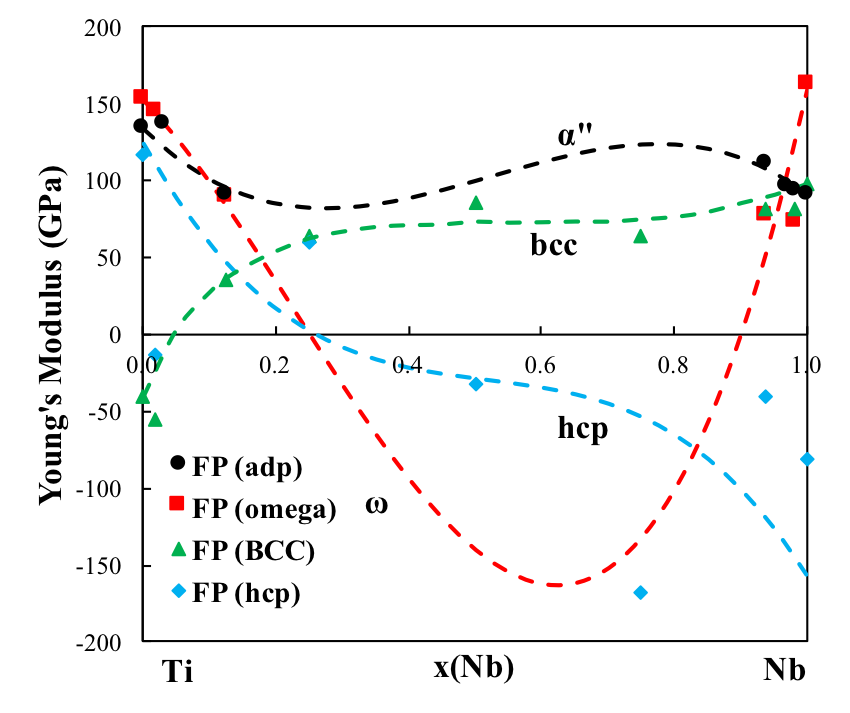
\includegraphics[width=\textwidth]{Chapter-7/Figures/tinbelastic.png}
	\caption{The elastic properites of the bcc, hcp, $\omega$, $\alpha"$ phases in the Ti-Nb system calculated from first-principles based on DFT are plotted as symbols. The CALPHAD fitting are plotted as the dashed lines. The figure is plotted from 100 at. \% Ti to 100 at. \% Nb.}
	\label{Ch7-figure:tinbelastic}
\end{figure}

\pagebreak
\begin{figure}[H]
	\centering
	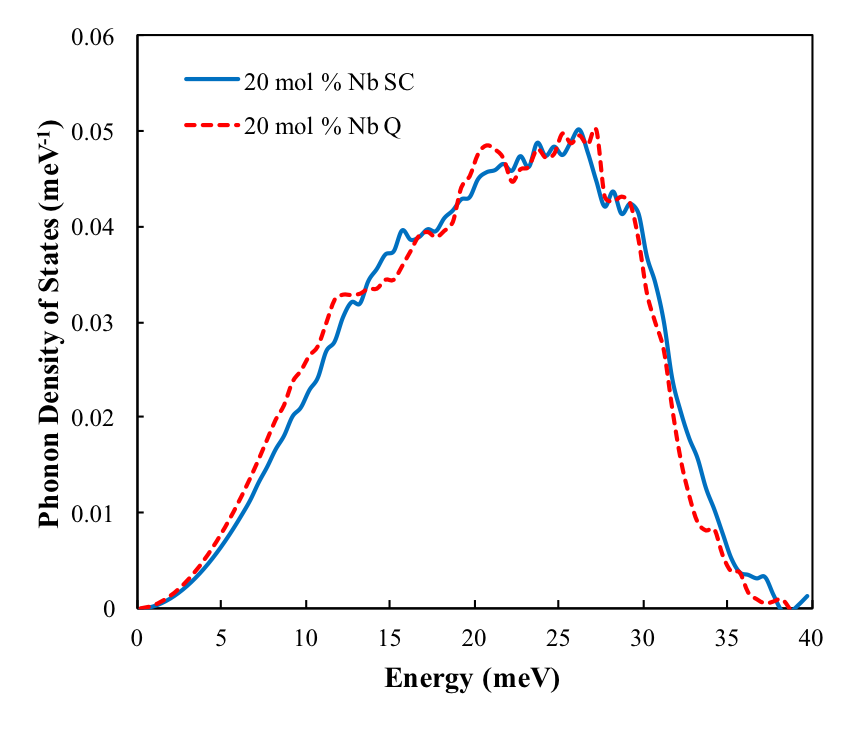
\includegraphics[width=\textwidth]{Chapter-7/Figures/50dos_20.png}
	\caption{The phonon density of states is plotted for the TiNb alloy at 20 at. \% Nb. The dashed line represents the slow cooled sample while the solid line represents the quenched sample.}
	\label{Ch7-figure:50dos_20}
\end{figure}

\pagebreak
\begin{figure}[H]
	\centering
	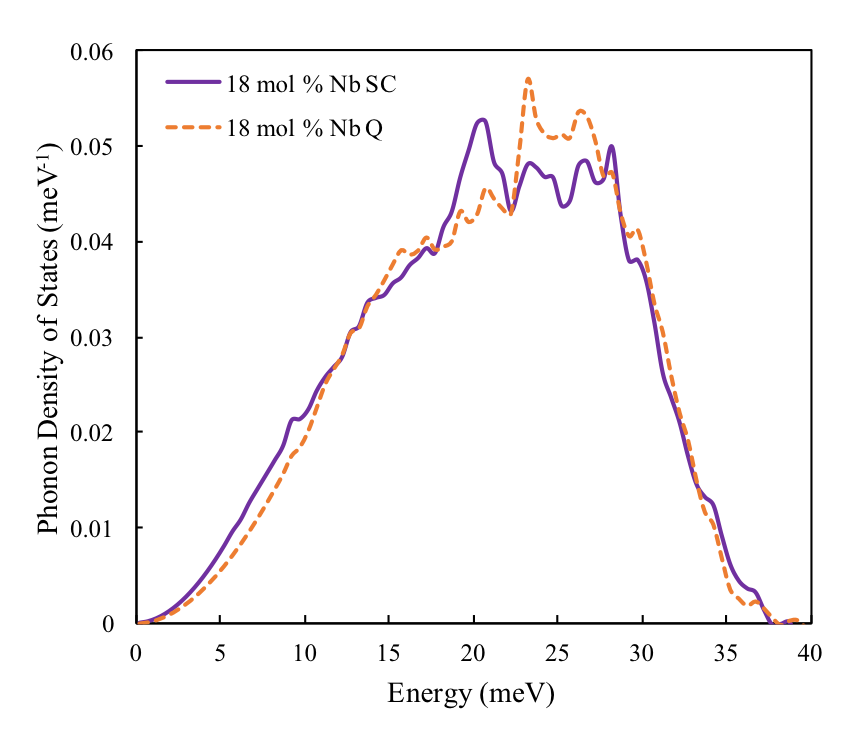
\includegraphics[width=\textwidth]{Chapter-7/Figures/50dos_18.png}
	\caption{The phonon density of states is plotted for the TiNb alloy at 18 at. \% Nb. The dashed line represents the slow cooled sample while the solid line represents the quenched sample.}
	\label{Ch7-figure:50dos_18}
\end{figure}

\pagebreak
\begin{figure}[H]
	\centering
	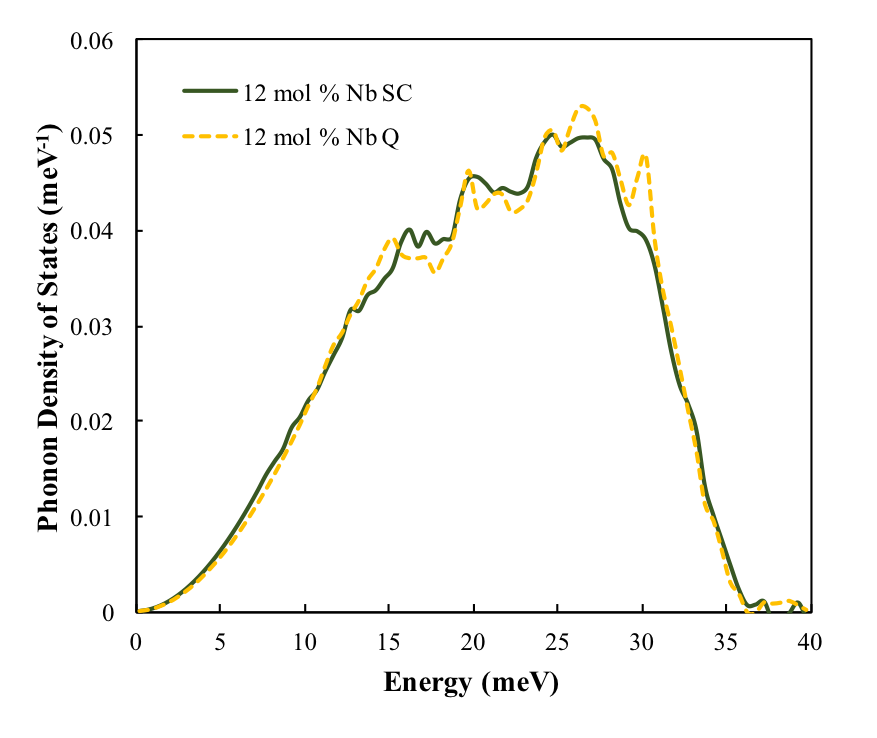
\includegraphics[width=\textwidth]{Chapter-7/Figures/50dos_12.png}
	\caption{The phonon density of states is plotted for the TiNb alloy at 12 at. \% Nb. The dashed line represents the slow cooled sample while the solid line represents the quenched sample.}
	\label{Ch7-figure:50dos_12}
\end{figure}

\pagebreak
\begin{figure}[H]
	\centering
	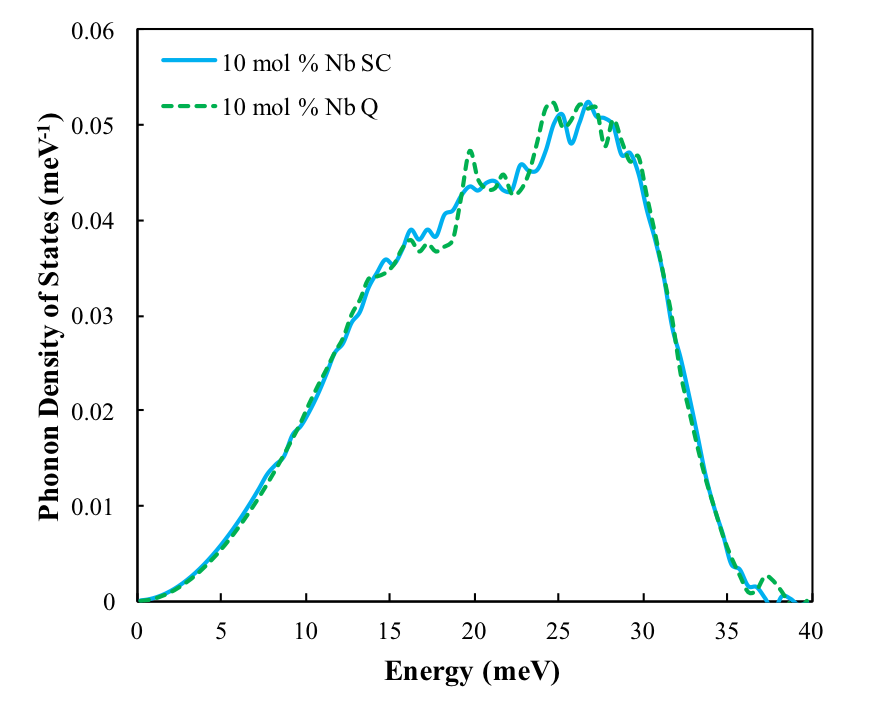
\includegraphics[width=\textwidth]{Chapter-7/Figures/50dos_10.png}
	\caption{The phonon density of states is plotted for the TiNb alloy at 10 at. \% Nb. The dashed line represents the slow cooled sample while the solid line represents the quenched sample.}
	\label{Ch7-figure:50dos_10}
\end{figure}

